\documentclass[11pt]{amsart}

\usepackage[a4paper,margin=1in]{geometry}
\usepackage{microtype}
\usepackage{amsmath,amssymb,mathtools}
\usepackage{graphicx}
\usepackage{booktabs}
\usepackage[colorlinks=true,linkcolor=blue,citecolor=blue,urlcolor=blue]{hyperref}

\title{Phase-A Results: The Free EMA-KL Surrogate Prevents Staleness Collapse,\\
and Its Theory Picks the Right Dose}
\author{Brian Bartoldson (experiments run and report drafted with Claude)}
\date{July 20, 2026}

\newcommand{\E}{\mathbb{E}}
\newcommand{\KL}{\mathrm{KL}}

\begin{document}
\maketitle

\begin{abstract}
Asynchronous RL trains on rollouts from stale policy snapshots; the free
EMA-KL surrogate $c\,(\log T_n - \log T_{n-\Delta})$ with
$c = \alpha/(\Delta(1-\alpha))$ regularizes against an implicit EMA anchor at
zero extra cost. On Qwen3-4B/Countdown (TBA, no centering) we find:
(1)~\textbf{without} the penalty, training \emph{collapses} at high staleness
--- homogeneous $\Delta{=}32$ falls from eval $0.75$ to $0.14$ by step 200, and
a heterogeneous mixture $\Delta_i \in \{1,4,10,32\}$ collapses $\sim$60 steps
later ($0.75 \to 0.002$ by step 300); (2)~\textbf{with} the penalty at the
theory-prescribed strength, every arm is stable and reaches eval
$0.79$--$0.83$; (3)~per-rollout calibration $c_i = \alpha/(\Delta_i(1-\alpha))$
matches the \emph{best} uniform dose found by a $3\times$ sweep
(peaks $0.816$ vs.\ $0.817$) --- calibration's value is that the theory
selects the right strength \emph{a priori}, without a sweep; the $3\times$
larger uniform dose costs $\sim$1.5 points. A homogeneous $\Delta{=}10$
reference through the new machinery reproduces the historical baseline
($0.829$ vs.\ $0.827$--$0.831$), and per-$\Delta$ telemetry confirms the
surrogate's predicted small-$\Delta$ variance (rel.\ error $5.9$ at
$\Delta\le2$ vs.\ $0.19$ at $\Delta\ge21$) without harming training.
(4)~Under symmetric NVFP4 emulation, quantization \emph{compounds} with
staleness: the FP4 $\Delta{=}32$, $\beta{=}0$ arm collapses ${\sim}70$ steps
earlier than its BF16 twin with a lower peak, while $\Delta{\lesssim}10$
stays stable; the \emph{same} theory dose $\beta c = 0.0045$ keeps $\Delta{=}10$
healthy and extends the $\Delta{=}32$ collapse boundary ${\sim}3\times$
(though not to full-horizon stability --- dose scaling for quantization is
untested). An asymmetric arm (BF16 trainer, FP4 sampler) fails informatively:
the un-centered quantization gap in the advantage-level penalty acts as a
global negative reward. (5)~In the original-hypothesis cell --- FP4 with
\emph{heterogeneous} staleness $\Delta_i \in \{1,4,10,32\}$ --- the
$\beta{=}0$ control collapses at ${\sim}$step 205 while both KL arms train
healthily through their full 24\,h horizons; on eval, per-rollout
staleness-weighted and uniform dosing \emph{tie} (peaks $0.771$ vs.\ $0.764$,
finals $0.771$ vs.\ $0.764$, single seed): the hypothesis's rescue claim
holds, but the weighting refinement is not separable from a well-chosen
uniform dose here.
\end{abstract}

\section{Setup}

All runs: Qwen3-4B-Instruct-2507 on Countdown with TBA (no centering,
importance sampling on), lr $10^{-6}$, $K{=}16$, seq.\ 4096, 720 target steps,
eval every 20 steps, $\alpha=0.9$, 2 nodes (4$\times$H100 inference /
4$\times$H100 training); 24\,h allocations (curves end at steps 490--690).
Configs in Appendix~\ref{app:configs}.

\paragraph{Heterogeneous staleness.} \texttt{--rl.staleness-offsets}
$o_{0..3}$ pins each of 4 data-parallel vLLM ranks to a fixed checkpoint lag
(reload every step to $\mathrm{step}-o_r$). $K$-groups stay
policy-homogeneous; training batches pool ranks and therefore mix policy ages
(verified in the rollout parquets: the trainer's step-10 batch carries
generating checkpoints $\{9,6,0,0\}$). The homogeneous arms use offsets
$10,10,10,10$ (reference) or the legacy reload rule at
\texttt{async\_level}$=$32 ($\beta{=}0$ control).

\paragraph{Anchors and calibration.} Every arm anchors both the importance
ratio and the KL term on the sampler's own vLLM logprobs. Per-rollout
calibration uses each sample's true lag: $c_i = \alpha/(\Delta_i(1-\alpha))$,
$\Delta_i \ge 1$; the uniform arms apply one dose $w = \beta\,c_{\mathrm{glob}}$
to every rollout ($c_{\mathrm{glob}} = 0.9/3.2 = 0.28125$). The per-token
clamp is in raw log-ratio units ($\pm 10$ before the coefficient), so
truncation is $\Delta$-invariant.

\paragraph{How the uniform constant was chosen (design decision).} The
uniform arms' primary constant was fixed by \emph{transporting} the
known-good effective strength from the homogeneous $\Delta{=}10$ baseline
($\beta c = 0.005 \times 0.9 = 0.0045$) and anchoring the global coefficient
at the \emph{maximum} staleness: $c_{\mathrm{glob}}$ uses
$\Delta_{\max} = 32$, and $\beta = 0.0045 / 0.28125 = 0.016$ so that
$\beta\,c_{\mathrm{glob}} = 0.0045$. This choice does \emph{not} account for
the fact that most lags in the $\{1,4,10,32\}$ mixture are below 32: because
the raw log-ratio magnitude grows roughly linearly in $\Delta_i$, a constant
raw weight yields an effective per-rollout dose $\propto \Delta_i/32$ ---
sub-maximal lags are effectively under-regularized relative to the
calibrated arm, whose effective dose is flat at $0.0045$ for every rollout.
Alternative constants (the mixture-mean-matched $w{=}0.015$ and the
$\Delta{=}1$-matched $w{=}0.045$) were run in the BF16 heterogeneous sweep
(Finding~2), where the $\Delta_{\max}$-anchored $w{=}0.0045$ performed best;
only that point was carried into the FP4 heterogeneous and within-group
batches.

\section{Results}

\begin{figure}[ht]
  \centering
  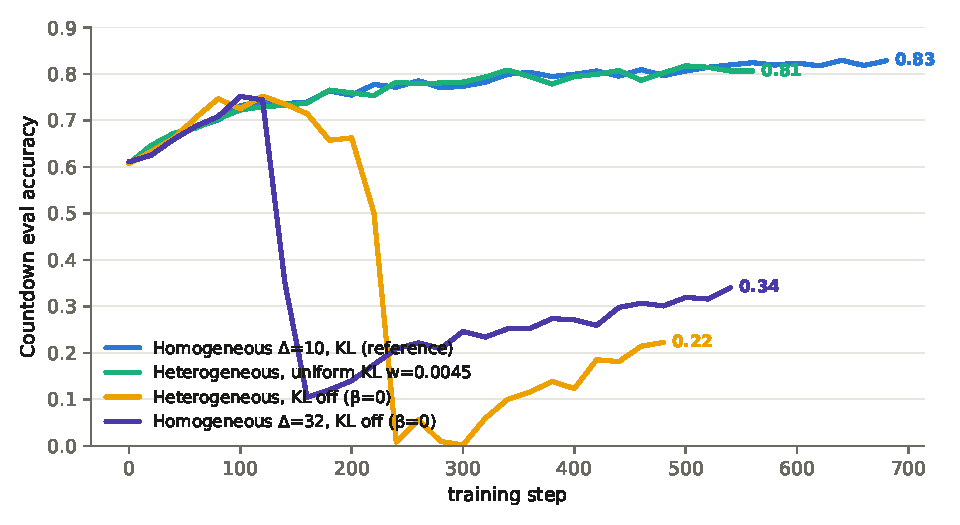
\includegraphics[width=0.92\linewidth]{fig_collapse_rescue.pdf}
  \caption{Collapse without the KL penalty; stability with it. Yellow
  (heterogeneous) and violet (homogeneous $\Delta{=}32$) are $\beta{=}0$:
  both collapse (steps ${\sim}230$ and ${\sim}170$) and never recover. Aqua
  (uniform dose $w{=}0.0045$) trains through the same window untouched; blue
  is the homogeneous $\Delta{=}10$ reference.}
  \label{fig:collapse}
\end{figure}

\paragraph{Finding 1: staleness alone collapses training; the free surrogate
prevents it.} The homogeneous $\Delta{=}32$, $\beta{=}0$ control peaks at eval
$0.752$ (step 100), then falls off a cliff between steps 160--180 (train
reward $0.68 \to 0.19$; eval $0.14$ at step 200) and oscillates around
$0.2$--$0.45$ for 400 more steps without recovering. The heterogeneous
$\beta{=}0$ control --- average lag $4\times$ smaller --- shows the same
failure delayed by ${\sim}60$ steps, preceded by a characteristic train-reward
overshoot ($0.94$ at step 127), then eval $0.002$ by step 300. Every arm with
the EMA-KL surrogate on, at any tested strength, trains stably through and far
beyond these windows. This is BF16 end to end: staleness alone, no
quantization, breaks unregularized async RL at these lags, and the
zero-cost surrogate fixes it.

\begin{figure}[ht]
  \centering
  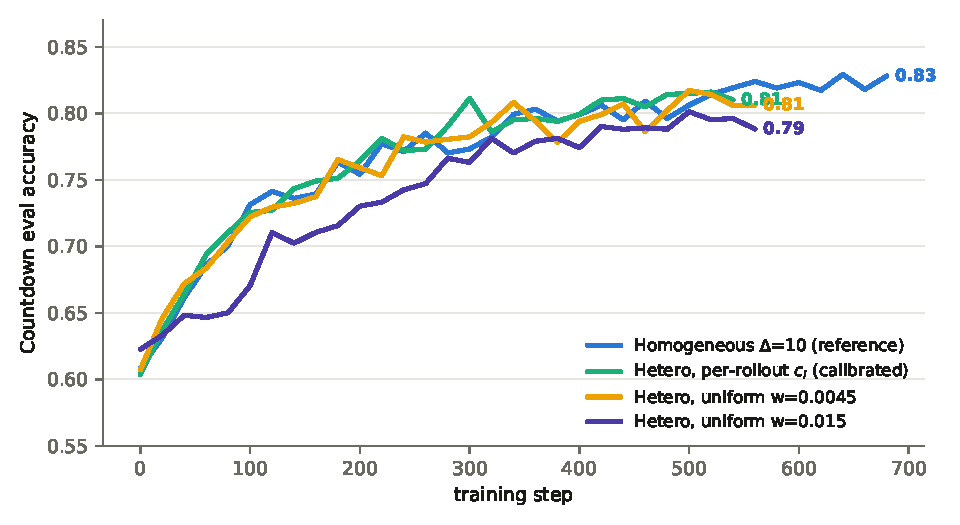
\includegraphics[width=0.92\linewidth]{fig_dose_calibration.pdf}
  \caption{All stable arms. Calibrated per-rollout $c_i$ (aqua) vs.\ the two
  uniform doses (yellow $w{=}0.0045$, violet $w{=}0.015$) under the same
  $\Delta_i \in \{1,4,10,32\}$ mixture; blue is the homogeneous reference.}
  \label{fig:dose}
\end{figure}

\paragraph{Finding 2: calibration matches the best swept dose --- without the
sweep.} Peaks: calibrated $0.816$ (step 520), uniform $w{=}0.0045$ $0.817$
(step 500), uniform $w{=}0.015$ $0.801$; reference $0.829$. The calibrated
arm and the best uniform arm are statistically indistinguishable at one seed,
and both sit ${\sim}1$ point under the homogeneous reference. Two honest
readings. First, on this task and $\Delta$ spread, per-rollout weighting adds
no \emph{performance} over the best \emph{tuned} uniform dose --- the
group-summed penalty appears to care mostly about total strength. Second, the
best uniform dose is exactly the one the theory prescribes
($w = \beta_{\mathrm{ref}} c_{\mathrm{ref}} = 0.0045$, transported from the
known-good homogeneous run via the $\beta c$ invariance), and tripling it
costs $1.5$ points: the calibration theory's practical payoff here is
\emph{dose selection without a sweep}, which is also what a practitioner
changing $\Delta$ (or mixing $\Delta_i$) actually needs.

\begin{figure}[ht]
  \centering
  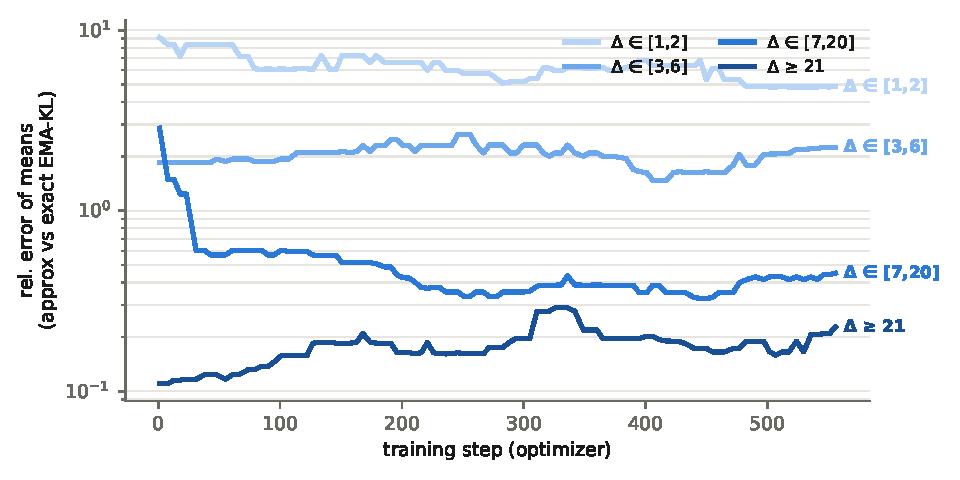
\includegraphics[width=0.92\linewidth]{fig_delta_strata.pdf}
  \caption{Relative error of the surrogate vs.\ exact EMA-KL by lag stratum
  (calibrated run; window-median smoothed; log scale).}
  \label{fig:strata}
\end{figure}

\paragraph{Finding 3: the surrogate's error is strongly $\Delta$-dependent
--- and training doesn't care.} Median rel.\ error of means: $5.88$
($\Delta\le2$), $2.13$ ($[3,6]$), $0.48$ ($[7,20]$), $0.19$ ($\ge 21$) ---
the theory note's finite-difference variance warning, measured. Despite a
quarter of tokens carrying rel.-error-${\sim}6$ estimates, the calibrated arm
matched the reference; the summed, $\beta$-scaled penalty is robust to
zero-mean estimator noise. Suggested refinement (untested): floor $\Delta_i$
at ${\sim}4$ in $c_i$.

\paragraph{Finding 4: mechanism and baseline controls.} The homogeneous
$\Delta{=}10$ reference through the full new machinery (offsets mechanism,
vLLM anchor, raw-units clamp) peaks $0.829$ / final $0.828$ --- inside the
historical no-centering band ($0.827$--$0.831$).

\section{FP4 results}

All FP4 arms use symmetric NVFP4 QDQ emulation (STE on trainer forwards, QDQ
on sampler checkpoints, bit-exact between the two) unless noted; same
Qwen3-4B/Countdown setup as above.

\begin{figure}[ht]
  \centering
  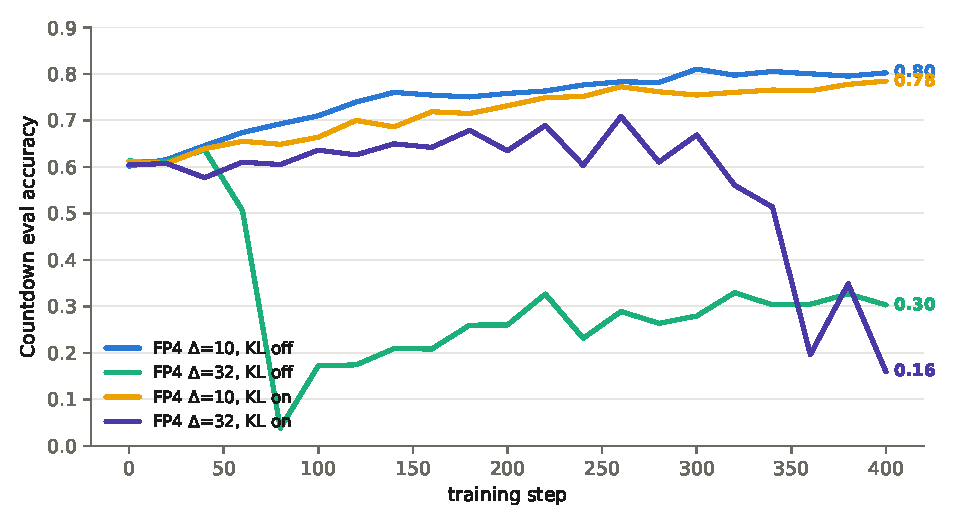
\includegraphics[width=0.92\linewidth]{fig_fp4.pdf}
  \caption{FP4 $\beta{=}0$ ladder and rescue arms. Blue/aqua: $\beta{=}0$ at
  $\Delta{=}10$ (stable) and $\Delta{=}32$ (collapses by step ${\sim}100$).
  Yellow/violet: the same theory dose $\beta c = 0.0045$ at $\Delta{=}10$
  (stable through 24\,h) and $\Delta{=}32$ (holds ${\sim}3\times$ past the
  $\beta{=}0$ boundary, degrades late).}
  \label{fig:fp4}
\end{figure}

\paragraph{Finding 5: quantization compounds with staleness, and the same
dose rescues it.} The $\beta{=}0$ ladder (Fig.~\ref{fig:fp4}): at
$\Delta{\approx}1$, FP4 training is stable and strong for 242 steps (train
reward $0.80$--$0.85$, eval $0.794$ at step 220; run ended early by a
data-loader file race, unrelated to training). At $\Delta{=}10$ it survives
its full 24\,h ($\sim$420 steps), volatile in train reward but climbing in
eval ($0.802$ at step 400). At $\Delta{=}32$ it collapses by step ${\sim}100$
(train reward $0.38$; eval already $0.17$) and stays collapsed ($0.303$ at
400). The BF16 twin at the same lag collapsed at step ${\sim}170$ from a
higher peak ($0.752$ vs.\ $0.637$): quantization and staleness
\emph{compound} --- the boundary moves ${\sim}70$ steps earlier and the
pre-collapse peak drops --- and at this horizon the $\beta{=}0$ boundary sits
between $\Delta{=}10$ and $32$. The rescue arms apply the \emph{same} theory
dose $\beta c = 0.0045$ used throughout, with no quantization-specific
retuning. At $\Delta{=}10$ this is fully sufficient: healthy through 24\,h,
eval $0.784$ at step 400. At $\Delta{=}32$ it carries training through and far
beyond the twin's collapse window ($0.636$ at 100, $0.679$ at 180, peak
$0.709$ at 260 --- a ${\sim}3\times$ extension of the boundary), but the
climb is slower and noisier at reduced altitude, and late in the 24\,h run
evals degrade ($0.51$ at 340 $\to$ $0.16$ at 400): the unscaled dose delays
rather than fully prevents the compounded failure. A quantization-aware dose
scaling (treating the quantization gap as extra effective staleness) is the
natural refinement --- untested.

\paragraph{Finding 6 (negative): the asymmetric arm fails informatively.}
The asymmetric arm (BF16 trainer, QDQ sampler, KL on at $\beta c = 0.0045$)
degrades monotonically from the start: eval $0.56$ at step 20, $0.04$ at 100,
$0.001$ by step 180; cancelled at 200. Mechanism: the surrogate's persistent
quantization gap enters the advantage-level (score-function) penalty
un-centered, acting as a global negative reward that suppresses all sampled
behavior --- not corrective QAT pressure. A differentiable KL-in-loss path,
or centering of the gap, would be needed for this setting.

\begin{figure}[ht]
  \centering
  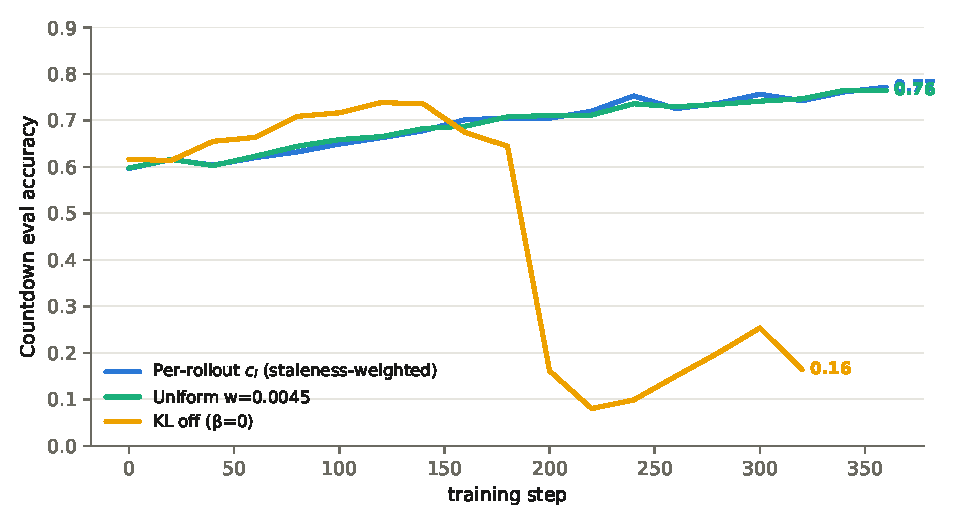
\includegraphics[width=0.92\linewidth]{fig_fp4hetero.pdf}
  \caption{The original-hypothesis cell: symmetric NVFP4 with heterogeneous
  staleness $\Delta_i \in \{1,4,10,32\}$. Yellow ($\beta{=}0$) collapses at
  ${\sim}$step 205 and never recovers; both KL arms --- per-rollout
  staleness-weighted $c_i$ (blue) and uniform $w{=}0.0045$ (aqua) --- train
  healthily through their full 24\,h horizons and end within $0.007$ eval of
  each other.}
  \label{fig:fp4hetero}
\end{figure}

\paragraph{Finding 7: the original-hypothesis cell --- staleness-weighted KL
under FP4 heterogeneity.} The batch that motivated this project: three arms,
all symmetric NVFP4 QDQ with the heterogeneous offsets
$\Delta_i \in \{1,4,10,32\}$ at \texttt{async\_level} 32 --- a $\beta{=}0$
control, a uniform dose $w{=}0.0045$ ($\beta{=}0.016$, global
$\Delta$-source), and per-rollout calibrated $c_i$ ($\beta{=}0.005$)
(Fig.~\ref{fig:fp4hetero}). The control collapses at ${\sim}$step 205 (train
reward $0.75$ at 140 $\to$ $0.51$ at 200 $\to$ $0.26$ at 212; eval $0.644$ at
180 $\to$ $0.161$ at 200) and never recovers through step 327 (eval $0.163$
at 320; the run ended early by a data-loader file race, unrelated to
training). The boundary at ${\sim}205$ sits between the FP4-homogeneous
$\Delta{=}32$ collapse (${\sim}100$) and the BF16-heterogeneous collapse
(${\sim}230$), consistent with an intermediate effective mismatch. Both KL
arms ran their full 24\,h with zero errors and ended healthy (final steps
${\sim}361$/$381$; last evals at step 360) --- notably, under the
heterogeneous mixture the uniform dose did \emph{not} reproduce the late
(${\sim}340$) degradation of its homogeneous-$\Delta{=}32$ counterpart; the
mixture's milder mean lag presumably explains it. The verdict on
staleness-weighting, from the eval curves: peaks $0.771$ (per-rollout, step
360) vs.\ $0.764$ (uniform, step 340), finals $0.771$ vs.\ $0.764$ at step
360 --- both gaps under $0.01$, a \emph{tie} at one seed, with the lead
trading at matched steps ($0.705$ vs.\ $0.711$ at 200; $0.756$ vs.\ $0.741$
at 300; $0.742$ vs.\ $0.746$ at 320). (Train reward frequently favored the
per-rollout arm --- e.g.\ $0.807$ vs.\ $0.735$ at 200 --- but that lead
traded on batch noise; we judge on evals.) Either way, the confirmed part
stands: staleness-weighted KL rescues FP4-heterogeneous training where
$\beta{=}0$ collapses --- the original hypothesis's rescue claim holds; the
comparison against uniform dosing is a tie at this seed count.

\section{Next steps}

Paired seeds ($\ge 3$) on calibrated vs.\ best-uniform; quantization-aware
dose scaling for the compounded mismatch (the $\Delta{=}32$ rescue's late
degradation suggests the unscaled dose is insufficient there); a
differentiable KL-in-loss path or gap-centered variant for the asymmetric
setting; dataloader retry-on-corrupt-parquet (the file race that ended the
async-1 arm); $\Delta_i$ floor test; a second task (MATH). Deferred items
and operational cautions are recorded in \texttt{EXPERIMENT\_ROADMAP.md} \S7
and \texttt{report\_fp4/OPERATIONS\_LOG.md}.

\appendix

\section{Configurations}\label{app:configs}

Common: \texttt{model=Qwen/Qwen3-4B-Instruct-2507}, \texttt{LR=1e-6},
\texttt{sampled\_k=train\_k=16}, \texttt{steps=720}, \texttt{type=tb},
\texttt{conf=COUNTDOWN.toml}, \texttt{seq\_length=4096},
\texttt{eval\_steps=20}, \texttt{reference\_mode=ema}, \texttt{ema\_alpha=0.9},
\texttt{kl\_centering=false}, \texttt{vllm\_logprobs=true}, batch 512, wandb
\texttt{fp4\_KL}, branch \texttt{fp4\_KL}.

\begin{center}
\small
\begin{tabular}{lllll}
\toprule
Arm & $\beta$ & async & offsets & $\Delta$-source \\
\midrule
\texttt{homog10\_approxKL\_b005\_vllmLP} & 0.005 & 10 & 10,10,10,10 & per\_rollout \\
\texttt{hetero\_approxKL\_b005\_perRollout} & 0.005 & 32 & 1,4,10,32 & per\_rollout \\
\texttt{hetero\_approxKL\_global\_w0045} & 0.016 & 32 & 1,4,10,32 & global \\
\texttt{hetero\_approxKL\_global\_w015} & 0.0533 & 32 & 1,4,10,32 & global \\
\texttt{hetero\_b0\_async32} & 0 & 32 & 1,4,10,32 & --- \\
\texttt{bf16\_b0\_async32} & 0 & 32 & --- (legacy rule) & --- \\
\texttt{fp4sym\_smoke} (60 steps) & 0.005 & 10 & --- & global \\
\texttt{fp4sym\_b0\_async1} & 0 & 1 & --- & --- \\
\texttt{fp4sym\_b0\_async10} & 0 & 10 & --- & --- \\
\texttt{fp4sym\_b0\_async32} & 0 & 32 & --- & --- \\
\texttt{fp4sym\_approxKL\_b005\_async10} & 0.005 & 10 & --- & global \\
\texttt{fp4sym\_approxKL\_b0016\_async32} & 0.016 & 32 & --- & global \\
\texttt{fp4asym\_approxKL\_b005\_async10}$^{\dagger}$ & 0.005 & 10 & --- & global \\
\texttt{fp4hetero\_b0\_async32} & 0 & 32 & 1,4,10,32 & --- \\
\texttt{fp4hetero\_approxKL\_global\_w0045} & 0.016 & 32 & 1,4,10,32 & global \\
\texttt{fp4hetero\_approxKL\_b005\_perRollout} & 0.005 & 32 & 1,4,10,32 & per\_rollout \\
\bottomrule
\end{tabular}
\end{center}

KL penalty: $-\beta \sum_t c\,\mathrm{clamp}(\log T_n - \log T_{n-\Delta},
\pm 10)$ added to advantages (no centering); $c$ per-token ($c_i$) or global
per the table. FP4 arms add \texttt{rollout\_quant=nvfp4} +
\texttt{fake\_quant=nvfp4} (252 patched linears; embeddings,
\texttt{lm\_head}, norms BF16). $^{\dagger}$BF16 trainer, QDQ sampler
(asymmetric; \texttt{fake\_quant} off).

\section{Eval table (selected steps)}

\begin{center}
\small
\begin{tabular}{lcccccc}
\toprule
Step & 100 & 200 & 300 & 400 & 500 & final \\
\midrule
Homog.\ $\Delta{=}10$ reference & 0.731 & 0.754 & 0.773 & 0.799 & 0.806 & 0.828 (680) \\
Hetero, per-rollout $c_i$ & 0.725 & 0.764 & 0.811 & 0.799 & 0.815 & 0.810 (540) \\
Hetero, uniform $w{=}0.0045$ & 0.722 & 0.759 & 0.782 & 0.794 & 0.817 & 0.806 (560) \\
Hetero, uniform $w{=}0.015$ & 0.670 & 0.730 & 0.763 & 0.774 & 0.801 & 0.788 (560) \\
Hetero, $\beta{=}0$ & 0.725 & 0.662 & 0.002 & 0.123 & --- & 0.222 (480) \\
Homog.\ $\Delta{=}32$, $\beta{=}0$ & 0.752 & 0.140 & 0.246 & 0.271 & 0.319 & 0.340 (540) \\
\midrule
FP4 $\Delta{\approx}1$, $\beta{=}0$ & 0.726 & 0.786 & --- & --- & --- & 0.779 (240) \\
FP4 $\Delta{=}10$, $\beta{=}0$ & 0.710 & 0.758 & 0.810 & 0.802 & --- & 0.802 (400) \\
FP4 $\Delta{=}32$, $\beta{=}0$ & 0.172 & 0.260 & 0.279 & 0.303 & --- & 0.303 (400) \\
FP4 $\Delta{=}10$, KL on & 0.664 & 0.731 & 0.755 & 0.784 & --- & 0.784 (400) \\
FP4 $\Delta{=}32$, KL on & 0.636 & 0.635 & 0.669 & 0.159 & --- & 0.159 (400) \\
FP4 asym.\ (BF16 trainer) & 0.036 & --- & --- & --- & --- & 0.001 (180) \\
FP4-hetero, $\beta{=}0$ & 0.716 & 0.161 & 0.254 & --- & --- & 0.163 (320) \\
FP4-hetero, uniform $w{=}0.0045$ & 0.659 & 0.711 & 0.741 & --- & --- & 0.764 (360) \\
FP4-hetero, per-rollout $c_i$ & 0.649 & 0.705 & 0.756 & --- & --- & 0.771 (360) \\
\bottomrule
\end{tabular}
\end{center}

\end{document}
